\chapter{Étude de l'asservissement de la MCC}

\section{Asservissement en courant}

\subsection{Modélisation sur Simulink}

A l'aide du PID Tuner de Simulink, nous obtenons les valeurs suivantes pour le correcteur PI :
\begin{itemize}
    \item $K_p = 5,68752963603813$
    \item $K_i = 52315,0706597655$
\end{itemize}

% image de l'asservissement en courant Simulink
\begin{figure}[H]
    \centering
    \includegraphics[width=1\textwidth]{images/BF_Courant/Schéma_Simulink_Asservissement_Courant.png}
    \caption{Schéma de l'asservissement en courant du moteur dans Simulink}
    \label{fig:asservissement_courant_simulink}
\end{figure}

\subsection{Modélisation sur PSIM}

Pour adapter le correcteur PI de Simulink à PSIM, il faut convertir les paramètres en utilisant les relations suivantes :

Dans Simulink : 
\[ G(s) = K_p + \dfrac{K_i}{s} = K_p \dfrac{s + \tfrac{K_i}{K_p}}{s} \]

Dans PSIM : 
\[ G(s) = k \dfrac{1 + sT}{sT} \Rightarrow k = K_p \text{ et } T = \dfrac{K_p}{K_i} \]

% image de l'asservissement en courant PSIM
\begin{figure}[H]
    \centering
    \includegraphics[width=1\textwidth]{images/BF_Courant/Schéma_PSIM_Asservissement_Courant.png}
    \caption{Schéma de l'asservissement en courant du moteur dans PSIM}
    \label{fig:asservissement_courant_psim}
\end{figure}

\subsection{Comparaison des résultats}

Dans cette section, nous allons comparer les résultats obtenus avec les deux outils de simulation, Simulink et PSIM.

% image de la comparaison des réponses
\begin{figure}[H]
    \centering
    \includegraphics[width=0.8\textwidth]{images/BF_Courant/Courbe_Comparaison_Asservissement_Courant.png}
    \caption{Comparaison des réponses indicielle de l'asservissement en courant du moteur entre Simulink et PSIM}
    \label{fig:comparaison_reponse_indicielle_courant}
\end{figure}

On constate que la réponse indicielle de l'asservissement en courant du moteur présente un dépassement d'environ 19\% et un temps de réponse de 0,35 ms. Ce qui respecte les spécifications du cahier des charges qui exige un dépassement maximal de 20\% et un temps de réponse maximal de 10 fois la prériode de la MLI soit 0,45 ms.


\section{Asservissement en vitesse}

\subsection{Simulation sur Simulink}
Nous commençons par la simulation de la vitesse du moteur en boucle ouverte sur Simulink. Nous réalisons le schéma suivant :

\begin{figure}[H]
    \centering
    \includegraphics[width=1\textwidth]{images/BO_Vitesse/Schéma_Simulink_BO_Vitesse.png}
    \caption{Schéma de la simulation en boucle ouverte de la vitesse du moteur dans Simulink}
    \label{fig:schéma_BO_vitesse_simulink}
\end{figure}

La simulation en boucle ouverte nous permet d'observer la réponse du système sans rétroaction. Pour cela, on attend d'être en régime permanent, pour lui appliquer en suite une consigne en échelon et observer la réponse du système.

\begin{figure}[H]
    \centering
    \includegraphics[width=0.8\textwidth]{images/BO_Vitesse/Graphe_BO_Vitesse.png}
    \caption{Réponse de la vitesse du moteur en boucle ouverte dans Simulink}
    \label{fig:asservissement_vitesse_simulink}
\end{figure}

On relève un temps de réponse à 5\% en boucle ouverte pour la vitesse, sur Simulink : 37,8 ms

Nous cherchons ensuite à asservir la vitesse du moteur en boucle fermée avec un correcteur PI. Nous visons un temps de réponse à 5\% 3 fois plus rapide qu'en boucle ouverte soit 12,6 ms avec un dépassement maximal de 20\%.
\begin{figure}[H]
    \centering
    \includegraphics[width=1\textwidth]{images/BF_Vitesse/Schéma_Simulink_BF_Vitesse.png}
    \caption{Schéma de l'asservissement en vitesse du moteur dans Simulink}
    \label{fig:asservissement_vitesse_simulink_schema}
\end{figure}

A l'aide du PID Tuner de Simulink, nous obtenons les valeurs suivantes pour le correcteur PI :

\begin{itemize}
    \item $K_p = 37,3376029909659$
    \item $K_i = 14022,585396076$
\end{itemize}

\subsection{Simulation sur PSIM}

\begin{figure}[H]
    \centering
    \includegraphics[width=0.8\textwidth]{images/BF_Vitesse/Schéma_PSIM_BF_Vitesse.png}
    \caption{Schéma de l'asservissement en vitesse du moteur dans PSIM}
    \label{fig:asservissement_vitesse_psim_schema}
\end{figure}



\subsection{Comparaison des résultats}

\begin{figure}[H]
    \centering
    \includegraphics[width=0.8\textwidth]{images/BF_Vitesse/Graphe_Comparaison_BF_Vitesse.png}
    \caption{Comparaison des réponses en vitesse entre Simulink et PSIM}
    \label{fig:comparaison_reponses_vitesse}
\end{figure}


Les deux courbes sont confondues, nous avons appliqué ici un facteur 0.99 sur les valeurs de vitesse issues de Simulink pour permettre de mieux visualiser les deux courbes.

\subsection{Asservissement en vitesse avec le codeur incrémental}
Le cahier des charges impose la possibilité d'asservir la vitesse du moteur à l'aide d'un codeur incrémental.

\subsubsection{Principe de fonctionnement du codeur incrémental}

Le fonctionnement du codeur incrémental repose sur un disque rotatif équipé de fentes. Celui-ci est interposé entre une diode électroluminescente et un capteur photodiode. Lorsque le disque tourne, les fentes permettent à la lumière de passer à travers, générant ainsi des impulsions électriques dans le capteur. Le nombre d'impulsions générées par tour dépend de la résolution du codeur.
\vspace{0.5cm}
Le codeur incrémental fournit est composé de deux pistes de fentes décalées d'un quart de période, ce qui permet de déterminer le sens de rotation du moteur en analysant la séquence des impulsions générées par les deux capteurs.
\subsubsection{Calcul de la vitesse et du sens de rotation}
Pour mesurer la vitesse de rotation du moteur, il suffit de compter le nombre d'impulsions générées par le codeur sur une période de temps donnée. La vitesse angulaire peut être calculée en utilisant la formule suivante :
\begin{equation}
    \omega = \frac{N \cdot 2\pi}{P \cdot T}
\end{equation}
où :
\begin{itemize}
    \item $\omega$ est la vitesse angulaire en radians par seconde (rad/s)
    \item $N$ est le nombre d'impulsions comptées
    \item $P$ est le nombre d'impulsions par tour du codeur
    \item $T$ est la période de temps pendant laquelle les impulsions sont comptées en secondes (s)
    \item $2\pi$ est une constante pour convertir les tours en radians
\end{itemize}

Pour connaitre le sens de rotation, on analyse la séquence des impulsions des deux pistes. Si la piste A précède la piste B, le moteur tourne dans un sens. Si la piste B précède la piste A, le moteur tourne dans le sens inverse.

\begin{figure}[H]
    \centering
    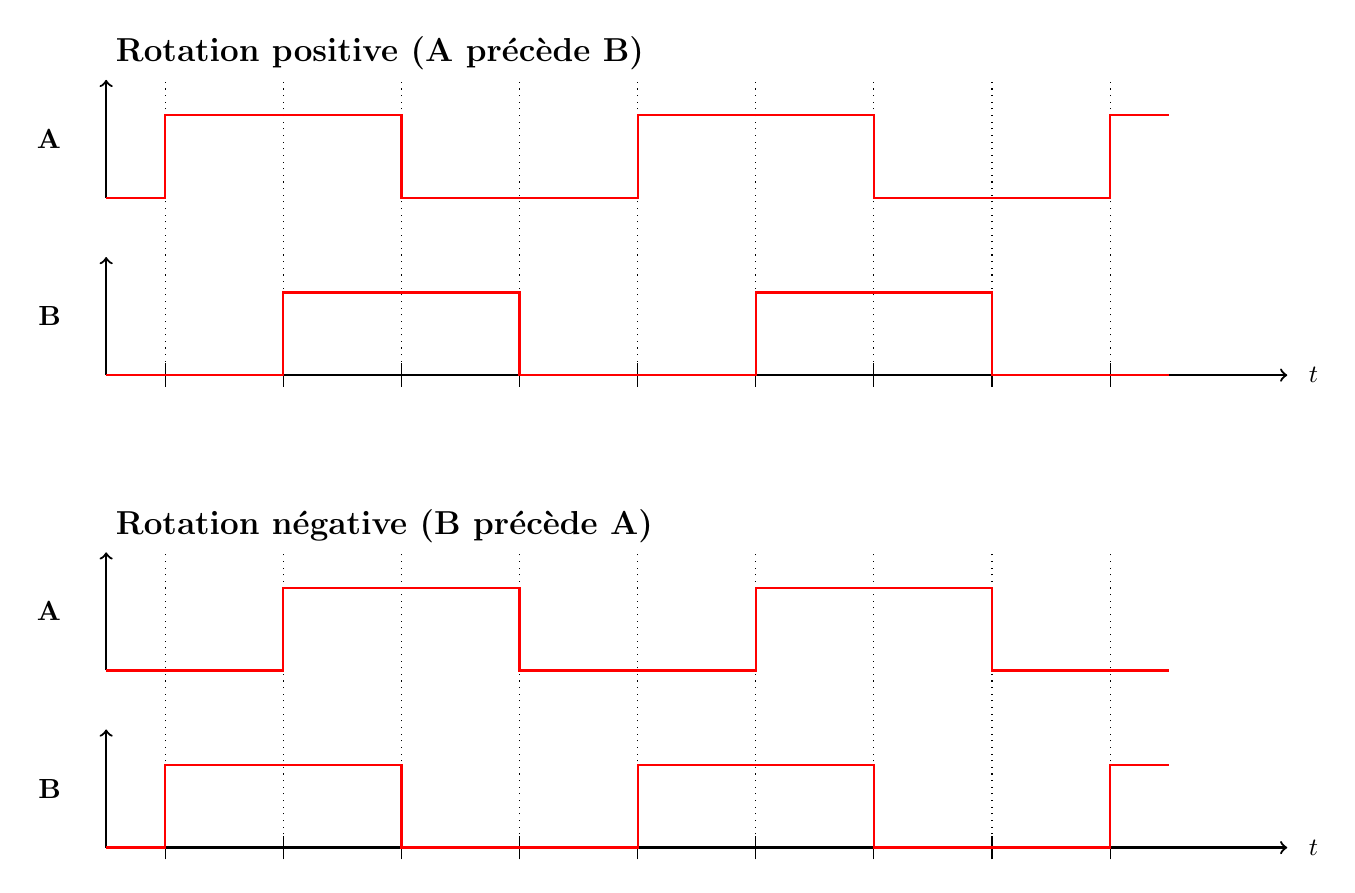
\begin{tikzpicture}[scale=1.5]
        % Titre Rotation positive
        \node[anchor=south west, font=\large\bfseries] at (0, 9) {Rotation positive (A précède B)};
        
        % Axe vertical pour A
        \draw[->, thick, black] (0, 8) -- (0, 9);
        \node[anchor=east] at (-0.3, 8.5) {\textbf{A}};
        
        % Axe vertical pour B
        \draw[->, thick, black] (0, 6.5) -- (0, 7.5);
        \node[anchor=east] at (-0.3, 7) {\textbf{B}};
        
        % Axe temps horizontal en bas
        \draw[->, thick, black] (0, 6.5) -- (10, 6.5);
        \node[anchor=west, font=\small] at (10.1, 6.5) {$t$};
        % Graduations et labels - alignées avec les fronts
        \draw[black] (0.5, 6.4) -- (0.5, 6.6);
        \draw[black] (1.5, 6.4) -- (1.5, 6.6);
        \draw[black] (2.5, 6.4) -- (2.5, 6.6);
        \draw[black] (3.5, 6.4) -- (3.5, 6.6);
        \draw[black] (4.5, 6.4) -- (4.5, 6.6);
        \draw[black] (5.5, 6.4) -- (5.5, 6.6);
        \draw[black] (6.5, 6.4) -- (6.5, 6.6);
        \draw[black] (7.5, 6.4) -- (7.5, 6.6);
        \draw[black] (8.5, 6.4) -- (8.5, 6.6);
        
        % Pointillés verticaux à chaque graduation
        \draw[dotted, thin, black] (0.5, 6.5) -- (0.5, 9);
        \draw[dotted, thin, black] (1.5, 6.5) -- (1.5, 9);
        \draw[dotted, thin, black] (2.5, 6.5) -- (2.5, 9);
        \draw[dotted, thin, black] (3.5, 6.5) -- (3.5, 9);
        \draw[dotted, thin, black] (4.5, 6.5) -- (4.5, 9);
        \draw[dotted, thin, black] (5.5, 6.5) -- (5.5, 9);
        \draw[dotted, thin, black] (6.5, 6.5) -- (6.5, 9);
        \draw[dotted, thin, black] (7.5, 6.5) -- (7.5, 9);
        \draw[dotted, thin, black] (8.5, 6.5) -- (8.5, 9);
        
        % Piste A - commence à 0 (en rouge) - premier front à t=0.5
        \draw[thick, red] (0, 8) -- (0.5, 8) -- (0.5, 8.7) -- (2.5, 8.7) -- (2.5, 8) -- (4.5, 8) -- (4.5, 8.7) -- (6.5, 8.7) -- (6.5, 8) -- (8.5, 8) -- (8.5, 8.7) -- (9, 8.7);
        
        % Piste B - commence à 0 (décalée de 1/4 de période, en rouge) - premier front à t=1.5
        \draw[thick, red] (0, 6.5) -- (1.5, 6.5) -- (1.5, 7.2) -- (3.5, 7.2) -- (3.5, 6.5) -- (5.5, 6.5) -- (5.5, 7.2) -- (7.5, 7.2) -- (7.5, 6.5) -- (9, 6.5);
        
        % Titre Rotation négative
        \node[anchor=south west, font=\large\bfseries] at (0, 5) {Rotation négative (B précède A)};
        
        % Axe vertical pour A
        \draw[->, thick, black] (0, 4) -- (0, 5);
        \node[anchor=east] at (-0.3, 4.5) {\textbf{A}};
        
        % Axe vertical pour B
        \draw[->, thick, black] (0, 2.5) -- (0, 3.5);
        \node[anchor=east] at (-0.3, 3) {\textbf{B}};
        
        % Axe temps horizontal en bas
        \draw[->, thick, black] (0, 2.5) -- (10, 2.5);
        \node[anchor=west, font=\small] at (10.1, 2.5) {$t$};
        % Graduations et labels - alignées avec les fronts
        \draw[black] (0.5, 2.4) -- (0.5, 2.6);
        \draw[black] (1.5, 2.4) -- (1.5, 2.6);
        \draw[black] (2.5, 2.4) -- (2.5, 2.6);
        \draw[black] (3.5, 2.4) -- (3.5, 2.6);
        \draw[black] (4.5, 2.4) -- (4.5, 2.6);
        \draw[black] (5.5, 2.4) -- (5.5, 2.6);
        \draw[black] (6.5, 2.4) -- (6.5, 2.6);
        \draw[black] (7.5, 2.4) -- (7.5, 2.6);
        \draw[black] (8.5, 2.4) -- (8.5, 2.6);
        
        % Pointillés verticaux à chaque graduation
        \draw[dotted, thin, black] (0.5, 2.5) -- (0.5, 5);
        \draw[dotted, thin, black] (1.5, 2.5) -- (1.5, 5);
        \draw[dotted, thin, black] (2.5, 2.5) -- (2.5, 5);
        \draw[dotted, thin, black] (3.5, 2.5) -- (3.5, 5);
        \draw[dotted, thin, black] (4.5, 2.5) -- (4.5, 5);
        \draw[dotted, thin, black] (5.5, 2.5) -- (5.5, 5);
        \draw[dotted, thin, black] (6.5, 2.5) -- (6.5, 5);
        \draw[dotted, thin, black] (7.5, 2.5) -- (7.5, 5);
        \draw[dotted, thin, black] (8.5, 2.5) -- (8.5, 5);
        
        \draw[thick, red] (0, 4) -- (1.5, 4) -- (1.5, 4.7) -- (3.5, 4.7) -- (3.5, 4) -- (5.5, 4) -- (5.5, 4.7) -- (7.5, 4.7) -- (7.5, 4) -- (9, 4);
        
        % Piste B - commence à 0 (B précède A, en rouge)
        \draw[thick, red] (0, 2.5) -- (0.5, 2.5) -- (0.5, 3.2) -- (2.5, 3.2) -- (2.5, 2.5) -- (4.5, 2.5) -- (4.5, 3.2) -- (6.5, 3.2) -- (6.5, 2.5) -- (8.5, 2.5) -- (8.5, 3.2) -- (9, 3.2);
        
    \end{tikzpicture}
    \caption{Chronogrammes selon le sens de rotation avec le codeur incrémental}
    \label{fig:chronogrammes_sens_rotation}
\end{figure}
